\tikzset{every picture/.style={line width=0.75pt}} %set default line width to 0.75pt        

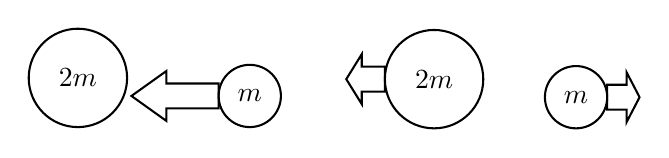
\begin{tikzpicture}[x=0.75pt,y=0.75pt,yscale=-.6,xscale=.6]
%uncomment if require: \path (0,420); %set diagram left start at 0, and has height of 420

%Shape: Circle [id:dp17026976972223973] 
\draw   (98,116.5) .. controls (98,94.68) and (115.68,77) .. (137.5,77) .. controls (159.32,77) and (177,94.68) .. (177,116.5) .. controls (177,138.32) and (159.32,156) .. (137.5,156) .. controls (115.68,156) and (98,138.32) .. (98,116.5) -- cycle ;
%Shape: Circle [id:dp1732786352755724] 
\draw   (250.5,131) .. controls (250.5,117.19) and (261.69,106) .. (275.5,106) .. controls (289.31,106) and (300.5,117.19) .. (300.5,131) .. controls (300.5,144.81) and (289.31,156) .. (275.5,156) .. controls (261.69,156) and (250.5,144.81) .. (250.5,131) -- cycle ;
%Left Arrow [id:dp2694928798272458] 
\draw   (180.5,131) -- (208.5,111) -- (208.5,121) -- (250.5,121) -- (250.5,141) -- (208.5,141) -- (208.5,151) -- cycle ;
%Shape: Circle [id:dp29195586713142996] 
\draw   (384,117.5) .. controls (384,95.68) and (401.68,78) .. (423.5,78) .. controls (445.32,78) and (463,95.68) .. (463,117.5) .. controls (463,139.32) and (445.32,157) .. (423.5,157) .. controls (401.68,157) and (384,139.32) .. (384,117.5) -- cycle ;
%Shape: Circle [id:dp47955008763043105] 
\draw   (512.5,132) .. controls (512.5,118.19) and (523.69,107) .. (537.5,107) .. controls (551.31,107) and (562.5,118.19) .. (562.5,132) .. controls (562.5,145.81) and (551.31,157) .. (537.5,157) .. controls (523.69,157) and (512.5,145.81) .. (512.5,132) -- cycle ;
%Left Arrow [id:dp529662098694889] 
\draw   (353,117.5) -- (365.4,97.5) -- (365.4,107.5) -- (384,107.5) -- (384,127.5) -- (365.4,127.5) -- (365.4,137.5) -- cycle ;
%Right Arrow [id:dp8432969383145832] 
\draw   (562.5,122) -- (578.1,122) -- (578.1,112) -- (588.5,132) -- (578.1,152) -- (578.1,142) -- (562.5,142) -- cycle ;

% Text Node
\draw (137.5,116.5) node   [align=left] {$\displaystyle 2m$};
% Text Node
\draw (275.5,131) node   [align=left] {$\displaystyle m$};
% Text Node
\draw (423.5,117.5) node   [align=left] {$\displaystyle 2m$};
% Text Node
\draw (537.5,132) node   [align=left] {$\displaystyle m$};


\end{tikzpicture}
